\documentclass{article}

%常规
\usepackage{geometry}
\usepackage{tikz}
%符号
\usepackage{amsmath}
\usepackage{amssymb}
\usepackage{physics}
\usepackage{graphicx}
%基础设置
\geometry{b5paper}
\linespread{1.5}
%个性化符号
%\newcommand{\dd}{\mathrm{d}}
\newcommand{\ii}{\mathrm{i}}
\newcommand{\ee}{\mathrm{e}}


\usepackage{newtxtext}
\usepackage{newtxmath}


\title{Introduction to Gauged Linear Sigma Models}
\author{Yilu Shao\\ \footnotesize{\it Institut de Mathématiques de Bourgogne, Université de Bourgogne Franche-Comté,}\\ \footnotesize{\it 9 avenue Alain Savary, Dijon, France}}
\date{}

\begin{document}

\maketitle

\begin{abstract}
    This is a note on 2d gauged linear sigma models presented by M. Romo in Fudan University. Based on Romo's review \cite{hori2014notes} with Hori. For related topics and new developments see \cite{Hori:2013ika} and \cite{Knapp:2020oba}.
\end{abstract}

\tableofcontents

\section{What is a GLSM?}
Actually for anyone who wants to know this, probably the best material is always Witten's groundbreaking work \cite{Witten:1993yc}...
\subsection{A Crash Course on 2d $\mathcal{N}=(2,2)$ SUSY Gauge Theories}
Generally a 2d $\mathcal{N}=(2,2)$ supersymmetric gauge theory contains the following matter contents:
\begin{itemize}
    \item \textit{Chiral multiplet} $(\phi,\overline{\phi},\psi,\overline{\psi},f,\overline{f},\ldots)$, in which $\phi,\overline{\phi}$ are complex scalars. $\psi,\overline{\psi}$ are complex spinors (superpartners) and $f,\overline{f}$ are auxilliary fields.
    \item \textit{Vectot multiplet} $(V_\mu,\lambda,\overline{\lambda},\sigma,\overline{\sigma},D)$$V_\mu$ are gauge (vector) fields. $\lambda,\overline{\lambda}$ are complex spinors (gauginos) and $\sigma,\overline{\sigma}$ are complex scalar fields. Special cares are to taken since $D$ is a \textbf{real} scalar field.
\end{itemize}
\subsection{A GLSM Dictionary}
A \textit{gauged linear sigma model} on flat space $\vvmathbb{R}^{1,1}$ or $\vvmathbb{R}^{2}$ is a 2d $\mathcal{N}=(2,2)$ supersymmetric gauge theory consists of the following data:
\begin{itemize}
    \item a compact Lie group $G$ called \textit{gauge group}
    \item $g_V:G\to\mathrm{GL}(V)$ a representation of $G$ called \textit{chiral module}
    \item a complex polynomial $\mathcal{W}:V\to \vvmathbb{C}$, called \textit{superpotential}
    \item $R:\mathrm{U}(1)_R\to\mathrm{GL}(V)$, called \textit{vector $R$-charge}
\end{itemize}
And the theory is controlled by a parameter called \textit{Fayet–Iliopoulos (FI) parameter}
\begin{equation*}
    t_i=\zeta_i-\ii\theta_i\in\vvmathbb{R}+\ii \frac{\vvmathbb{R}}{2\pi\vvmathbb{Z}},\quad i=1,...,s,\;s=\mathrm{rank}(\mathrm{Lie}(G))
\end{equation*}
Here we only consider the \textit{abelian} GLSMs, the gauge group looks like $\mathrm{U}(1)^s$ in which the \textit{rank} is just $s$. For nonabelian case we have, for example
\begin{equation*}
    G=\mathrm{U(N)\sim \mathrm{U}(1)\times\mathrm{SU}(N)}\leadsto s=1.
\end{equation*}
Now we can write down the action for an (abelian) GLSM:
\begin{equation}
    S_{\mathrm{GLSM}}=S_{\mathrm{kin.}}+S_{\mathrm{gauge,kin.}}+S_{W}+S_{\mathrm{FI}}
\end{equation}
Each term has:
\begin{itemize}
    \item kinematic terms of chiral fields $\abs{\partial\phi}^2 \in S_{\mathrm{kin.}}$ completely fixed by SUSY.
    \item kinematic terms of gauge fields $\operatorname{Tr}{F}^2 \in S_{\mathrm{gauge,kin.}}$, with $F_V=\partial_{[\mu}V_{\nu]}$. Also completely fixed by SUSY.
    \item $S_{W}$ and $S_{\mathrm{FI}}$ contain free parameters or couplings.
\end{itemize}
The explicit forms of $S_W$ (called \textit{superpotential}) is 
\begin{equation}
    S_W=\int_{\vvmathbb{R}^2}(-\frac{\ii}{2}f^{\alpha}\partial_{\alpha}W-\frac{\ii}{2}\overline{f}^{\Dot{\alpha}}\overline{\partial}_{\Dot{\alpha}})+\text{(fermion\ terms)}.
\end{equation}
And $S_{\mathrm{FI}}$ (called \textit{twisted potential}) is
\begin{equation}
    S_{\mathrm{FI}}=\int_{\vvmathbb{R}^2}(-\frac{\ii}{2\pi}\sum_{i}\zeta^{i}D_i-\frac{\ii}{2\pi}\sum_{i}\theta_i F_V^i).
\end{equation}
the dot here denotes different chirality, using van der Waerden notation \cite{Wess:1992cp}.

We also note that:
\begin{enumerate}
    \item Different $\phi_\alpha$ corresponds to different $f_\alpha$.
    \item The FI parameters $t_i=\zeta_i-\ii\theta_i\in \mathscr{M}_K$ make up the moduli space of a GLSM, and the $K$ got its name from \textit{K\"{a}hler}.
\end{enumerate}

\subsection{Constraints on Superpotential and Anomalies}
While $\mathcal{W}$ will actually determine the properties of the 2d theory, there are certain constraints on the form of $\mathcal{W}$.

First is gauge invariance


\subsection{LG/CY Correspondence in GLSM: An Example}
\begin{figure}[htbp]
	\centering
	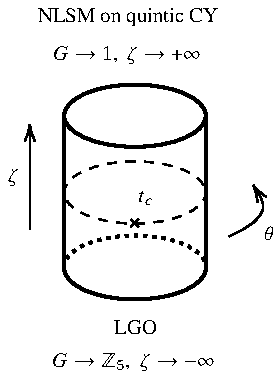
\includegraphics{LG-CY.pdf}
	\caption{Phases of a GLSM.}
	\label{fig:ospquiver}
\end{figure}



\nocite{Hori:2000ck,Hori:2003ic,Hori:2000kt,Hori:2006dk,Hori:2002,Hori:2016}
\bibliographystyle{amsalpha}
\bibliography{main.bib}

\end{document}
